% Implementation

\chapter{Introduction}
\label{ch:impl_introduction}


Before dealing with the models themselves we have been trying to find
the best way to select a feature subset for the prediction of the
\textit{Bitcoin} price. We used two methods. First \textit{principal
component analysis (PCA)}, an then \textit{wrapper FSS (WFSS)} both
presented in \autoref{ch:feature-selection}.

For \textit{PCA} we used a \textit{Python} implementation included in
the library \textbf{scikit-learn}. On the other hand, for
\textit{WFSS} we have built it to embed the models inside it in order
to select the right subset of features.

To run the needed experiments to compare the two models studied we
searched for a way to build both \textit{recurrent neural networks
(RNN)} and \textit{vector autoregressions (VAR)}, for which we have
used \href{http://www.keras.io}{Keras} and \textbf{vars} package.
\href{http://www.keras.io}{Keras} is an open source neural network
library written in \textit{Python}. Designed to enable fast
experimentation with deep neural networks, it focuses on being
minimal, modular and extensible. The \textbf{vars} package is a
library of programming functions for the \textit{R programming
language} which provides an implementation of vector autoregressive,
structural vector autoregressive and structural vector error
correction models as well as functions for diagnostic testing,
estimation of a restricted models, prediction, causality analysis,
impulse response analysis and forecast error variance decomposition.

For the assessment of the two models we developed \textit{time series
cross-validation (TSCV)} which is an adaptation of
\textit{cross-validation} for time series prediction assessment.

\chapter{Time Series Cross Validation}
\label{ch:tscv}

\textit{Time series cross validation (TSCV)} is a model validation
technique for assessing how the results generalize to an independent
data set. It derives from \textit{cross-validation} which is also a
model validation technique that is used for \textit{cross-sectional}
data. \textit{Cross-validation} partitions the given dataset in two
disjoint subsets of the examples present in the dataset. They are
called \textit{train partition} and a \textit{test partition}. The
prediction model is built with the \textit{train partition} elements
and later it's accuracy is measured using the \textit{test partition}
elements. This operation can be performed many times with selecting
different examples for the \textit{train-test} partitions, to later
average the accuracy measures obtained in each iteration of model
prediction and model assessment. This techniques helps us avoid
overfitting and to have an insight on how will the model generalize to
an independent dataset with unknown data.

A particular case of \textit{cross-validation} that \textit{TSCV} is
based on is called \textit{leave-one-out cross-validation (LOOCV)}.
The distinctive feature of \textit{LOOCV} is that the \textit{test
partition} is composed of only one element of the dataset, while the
\textit{train partition} is composed of $D - 1$ elements, beeing $D$
the size of the dataset. This technique is used when there is a need
to reduce computations due to the possible combinations of
\textit{train-test partitions}, because \textit{LOOCV} builds $D$
models with their respective validation.

Now we get to \textit{time-series cross-validation} which was proposed
by \cite{hart1994automated} as a way to get the same properties that
\textit{cross-validation} offers for \textit{cross-sectional} data
applied to \textit{time-series} data. \textit{Time-series} data is
characterized by the sequence that it's elements form, the elements of
a \textit{time-series} are always present in the same order, they have
sequential dependency one with the previous and next elements. Another
feature of \textit{time-series} as an ordered sequence of events is
that there isn't a point in predicting a past event given. In other
words, given a $y^{(t)}$ there is a interest in predicting $y^{(t+k)},
k \in \{1,\dots,N\}$ but not much in predicting $y^{(t-k)}, k \ in
\{1, \dots, N\}$. Added to that, the models that deal with
\textit{time-series} take advantage of their property by enforcing the
sequential dependencies in their formulation, hence we can not present
the elements of the dataset in any sequence, we have to present them
in the correct order by which they are created or observed.

Given all the constraints, i.e. that we want to maintain the right
order of the samples, and use \textit{LOOCV}, partition the data again
in \textit{train partition} and \textit{test partition}. The
difference with standard \textit{LOOCV} is that the \textit{train
partition} is composed of contiguous \textit{time-series} elements,
usually starting from the $1$-st and ending with the $(T - i)$-th
element, where $T$ is the size of the \textit{time-series} and $i$ is
a decreasing value, which initial value is a parameter that depends on
the problem domain and the model been assessed. Then the \textit{train
partition} is a one element set composed by the $(T - i + 1)$-th
element. Another difference that arose from this explanation, is that
in \textit{TSCV} there are certain \textit{train-test partition}
configuration where part of the elements of the \textit{time-series}
are not been selected.

Let's look at the example of \autoref{fig:tscv-example} assuming that
is reflecting the initial partition. The size of the
\textit{time-series} is $T = 41$, composed of \textit{train partition}
represented by the red dots, \textit{test partition} represented by
the green triangle and non selected elements represented by the blue
dots. Here the \textit{train partition} is composed of all the
elements that go from the $1$-st to the $10$-th. Here $i$ has an
initial value of $31$, so the last element of the \textit{train
partition} is $T - i = 41 - 31 = 10$-th. The \textit{test partition}
is the $T - i + 1 = 41 - 31 + 1 = 11$-th element. This way, the
\textit{train-test partition} would incrementally include more and
more elements of the \textit{time-series} until reaching the last one
as shown in \autoref{eq:tscv-example}.

\begin{equation}
  \begin{aligned}
    \label{eq:tscv-example}
    \{1,\dots,10\} & \{11\} \\
    \{1,\dots,11\} & \{12\} \\
    &\vdots \\
    \{1,\dots,39\} & \{40\} \\
    \{1,\dots,40\} & \{41\} \\
  \end{aligned}
\end{equation}

\begin{figure}[bth]
  \myfloatalign
  {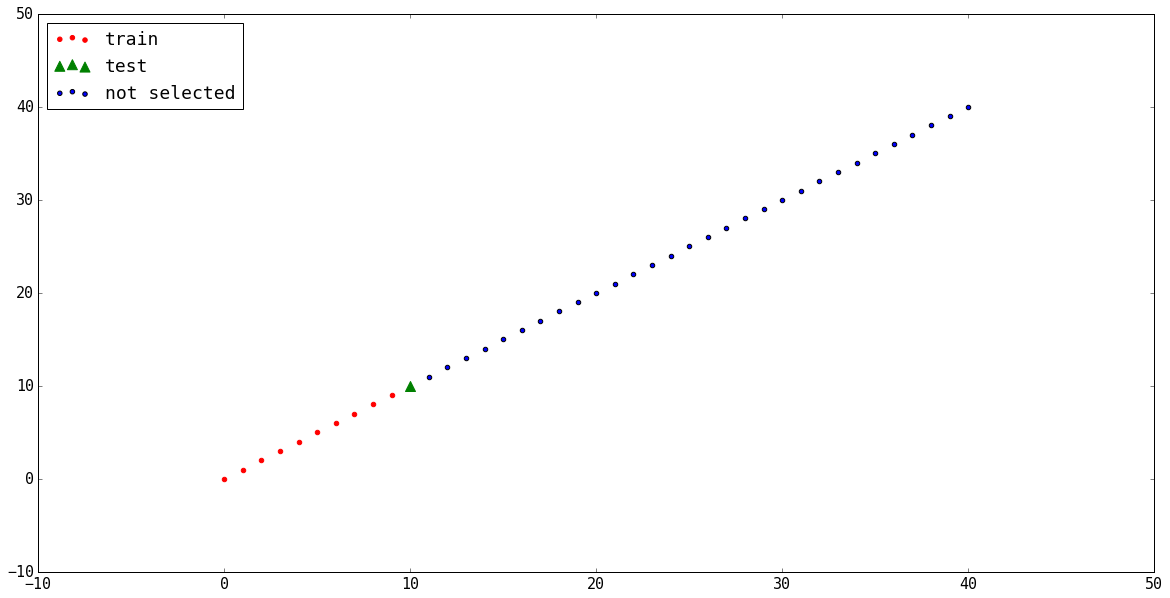
\includegraphics[width=1\linewidth]
    {gfx/tscv-example}}
  \caption{\textit{Time series cross validation} example}
  \label{fig:tscv-example}
\end{figure}

In \autoref{lst:tscv-pseudo-code} we summarize in a
\textit{Python}-like pseudo-code the behavior of \textit{TSCV}.

\begin{code}[language = Python, frame = single,
  caption = {\textit{TSCV} pseudo code},
  label = lst:tscv-pseudo-code,
  captionpos = b][bth]
def tscv(dataset, model):
  overall_error = 0
  start = 0
  end = 10 
  test_pos = 11

  T = 41

  for i in range(train_end, T):
    train_part, test_part = dataset.get_parts(start, end,
                                              test_pos)
    result = model.fit(train_part)
    error = asses_model(test_part, result)
    overall_error = aggregate_error(overall_error, error)

    end = i
    test_pos = i + 1

  return overall_error
\end{code}

\chapter{Wrapper Feature Subset Selection}
\label{ch:wfss}

\textit{Feature subset selection} techniques are divided in two
categories \textit{filter} techniques and \textit{wrapper} techniques.
\textit{Filter} techniques are applied over the dataset to extract the
features an give the same \textit{feature subset} as result regardless
of the model used in the prediction process. One example of this
category es \textit{principal component analysis}. On the other hand,
wrapper techniques are applied embedding the model in the assessment
process of the \textit{feature subset} selected. Basically a
\textit{feature subset} is selected, then a model is fitted to to that
subset. Then the model is assessed and compared to another
\textit{feature subset}.

We have used \textit{wrapper feature subset selection (WFSS)}
introduced by \cite{kohavi1997wrappers}. We used a variant of
\textit{WFSS} that reduces the search space by using a greedy strategy
to find the \textit{feature subset selection}. This version of
\textit{WFSS} doesn't guarantee to get the subset with the best
performance, however it gets a good result in less time.
\autoref{lst:wfss-pseudo-code} describes with a \textit{Python}-like
pseudo code how the version of \textit{WFSS} we've implemented works.

\begin{code}[language = Python, frame = single,
  caption = {\textit{WFSS} pseudo code},
  label = lst:wfss-pseudo-code,
  captionpos = b][bth]
def wfss(dataset, model):
  not_sel = dataset.get_features() # Not selected features
  sel = [] # Selected features
  overall_error = *infinity* # Assign a big number
  
  while not is_empty(not_sel):
    # Select candidate
    cand_error = *infinity* # Assign a big number
    for cand in not_sel:
      new_error = assess_features(concat(sel, cand))
      if cand_error > new_error:
        selected_candidate = cand
        cand_error = new_error

    if not overall_error > new_error:
      # Stop if the new candidate doesn't
      # improve the assessment of the
      # previously selected candidates
      break
    else:
      overall_error = new_error
      sel.append(selected_candidate)
      not_sel.remove(selected_candidate)

  return sel
\end{code}

% Present the pseudo-code and then a Python version without all the
% details

        % while not_selected_vars:
        %     score = sys.maxsize
        %     selected_var = ''

        %     for col in not_selected_vars:
        %         # pdb.set_trace()
                
        %         candidate_columns = selected_vars.copy()
        %         candidate_columns.append(col)
                
        %         X,y = dataset.get_columns(columns = candidate_columns)

        %         candidates_score = tscv_score(X,y)

        %         print("Candidate columns: ", candidate_columns)
        %         print("Candidates score: ", candidates_score)
                
        %         if candidates_score < score:
        %             score = candidates_score
        %             selected_var = col

        %     if score < selected_vars_score:
        %         selected_vars.append(selected_var)
        %         not_selected_vars.remove(selected_var)
        %         selected_vars_score = score

        %         print("Selected vars: ", selected_vars)
        %         print("Current MAE: ", selected_vars_score)
        %     else:
        %         break


%---------------------------------------------------------------------
%---------------------------------------------------------------------
%---------------------------------------------------------------------

%\enlargethispage{2cm}

%------------------------------------------------

%%% Local Variables:
%%% mode: latex
%%% TeX-master: "../main"
%%% End:
